\begin{chapter}{Some examples}
After introducing a method to produce a QP associated to an arbitrary polygonal subdivision of a surface, a natural question arises: is the associated Jacobian algebra always finite-dimensional? As shown in \cite{Lad12}, this is indeed the case for triangulations of closed surfaces. In this section, we will show that this is not true for arbitrary subdivisions. In fact, we will produce examples of both finite and infinite-dimensional algebras arising from subdivisions of closed surfaces of every genus.
\begin{section}{A family of finite-dimensional examples}

We start by showing that surfaces of any genus admit a particular decomposition into disjoint disks.

A \emph{loop} $f$ on a surface $\Sigma$ is a smooth embedding $f:S^1\to \Sigma$. We will identify a loop with its image on $\Sigma$. A \emph{handle} is a torus with a disk removed. We recall that a surface of genus $g>0$ can be obtained starting with a disk with $g-1$ holes and gluing handles along each hole and the boundary of the disk. \textcolor{red}{[citation needed]}

\begin{figure}[h]
\centering
	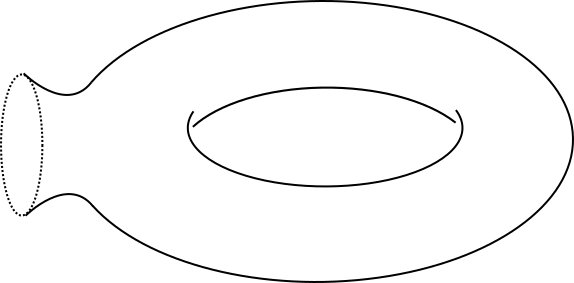
\includegraphics[width=0.5\textwidth]{handle.png}
\caption{A handle.}
\end{figure}

\begin{prop}\label{surface-loops} Let $\Sigma$ be a surface of genus $g$. There exist finite families $R=\{r_i\}$ and $B=\{b_j\}$ of loops on $\Sigma$ such that:
\begin{enumerate}
\item Two loops in the same family are disjoint.
\item Any point of the surface belongs to at most two loops.
\item The loops divide the surface into a disjoint family of regions, each of them a disk (up to homeomorphism).
\end{enumerate}
\end{prop}

\begin{proof} We give an explicit construction of such families.

The case in which $g=0$ (the sphere) is easily dealt with by choosing a single loop $r_1$ as the equator, since both hemispheres are homeomorphic to a disk and the other conditions are vacuously true.

For the cases in which $g>0$, we will make use of the handle decomposition we mentioned previously. We will draw a handle as a square (with opposite edges identified) having a gray hole in its center. Consider the following configuration:

\begin{figure}[h]
\[
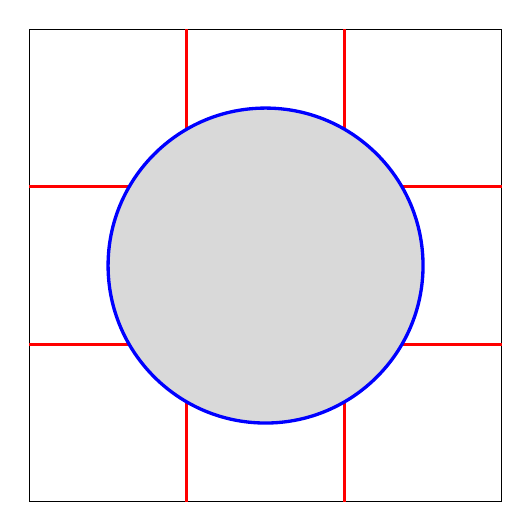
\begin{tikzpicture}
\draw (0,0) node[minimum size=6cm,draw] {};

\fill [black,opacity=.15] circle (2cm);

\draw[red, very thick] (-3,1) -- (-1.73,1);
\draw[red, very thick] (-3,-1) -- (-1.73,-1);

\draw[red, very thick] (3,1) -- (1.73,1);
\draw[red, very thick] (3,-1) -- (1.73,-1);

\draw[red, very thick] (1,-3) -- (1,-1.73);
\draw[red, very thick] (-1,-3) -- (-1,-1.73);

\draw[red, very thick] (1,3) -- (1,1.73);
\draw[red, very thick] (-1,3) -- (-1,1.73);

\draw[blue, very thick] (0,0) circle (2cm);
\end{tikzpicture}
\]
\end{figure}

We first deal with the case in which $g=1$. If we glue such a handle to the boundary of the following disk, we obtain a torus with a single red loop $r_1$ and a single blue loop $b_1$:

\begin{figure}[h]
\label{divided-handle}
\[
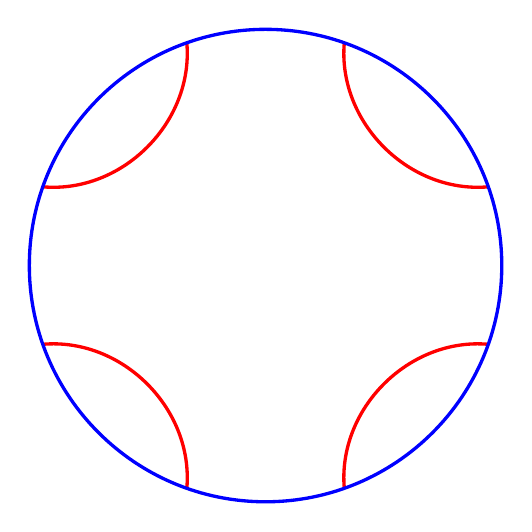
\begin{tikzpicture}

\draw[red, very thick] (-2.83,1) to [bend right=50] (-1,2.83);
\draw[red, very thick] (2.83,1) to [bend left=50] (1,2.83);
\draw[red, very thick] (2.83,-1) to [bend right=50] (1,-2.83);
\draw[red, very thick] (-2.83,-1) to [bend left=50] (-1,-2.83);

\draw[blue, very thick] (0,0) circle (3cm);
\end{tikzpicture}
\]
\end{figure}

Once again, the intersection conditions are vacuous. Finally, we observe that the blue loop cuts the torus into a disk and a handle, so one can check condition $3$ in both objects separately. One sees at once that the disk gets cut up into 5 smaller disks, while the handle is divided into $3$ disks, as we wanted.

While the solution to the case $g=1$ may be easier to draw directly on a square instead of considering a handle decomposition, the latter helps to illustrate the general case, which we now consider. For the case $g>1$, we regard our surface as a disk with $g-1$ holes, with a handle divided as in \ref{divided-handle} attached to its boundary and to each of its holes. We now exemplify the configuration on the \textcolor{red}{holed} disk for $g=4$:

\begin{figure}[h]
\[
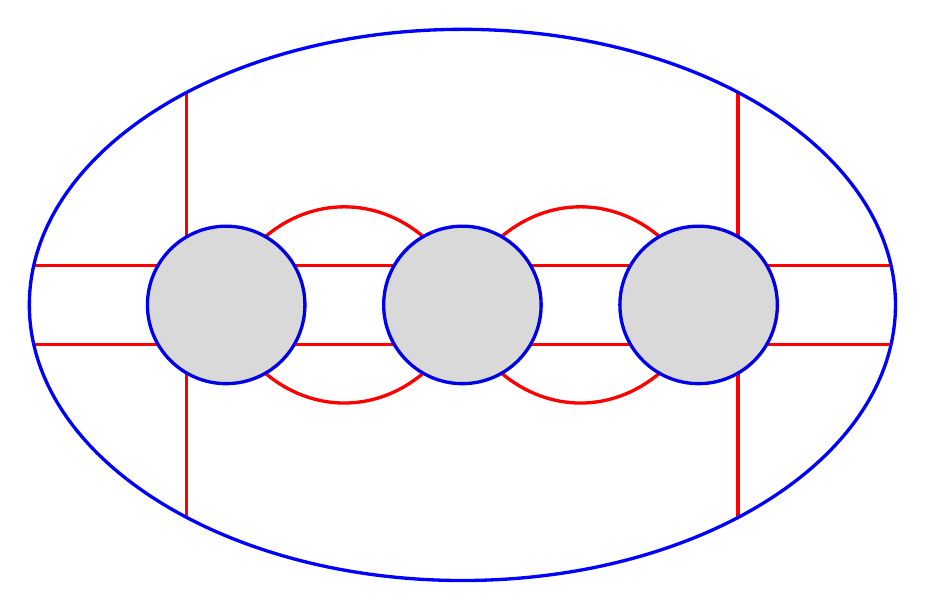
\begin{tikzpicture}
\draw[red, very thick] (-5.44, 0.5) -- (-3.87, 0.5);
\draw[red, very thick] (-5.44, -0.5) -- (-3.87, -0.5);
\draw[red, very thick] (5.44, 0.5) -- (3.87, 0.5);
\draw[red, very thick] (5.44, -0.5) -- (3.87, -0.5);

\draw[red, very thick] (-3.5,0.87) -- (-3.5,2.7);
\draw[red, very thick] (-3.5,-0.87) -- (-3.5,-2.7);
\draw[red, very thick] (3.5,0.87) -- (3.5,2.7);
\draw[red, very thick] (3.5,-0.87) -- (3.5,-2.7);

\draw[red, very thick] (-2.137, 0.5) -- (-0.863, 0.5);
\draw[red, very thick] (-2.137, -0.5) -- (-0.863, -0.5);
\draw[red, very thick] (2.137, 0.5) -- (0.863, 0.5);
\draw[red, very thick] (2.137, -0.5) -- (0.863, -0.5);

\draw[red, very thick] (-2.5,0.87) to [bend left=40] (-0.5,0.87);
\draw[red, very thick] (2.5,0.87) to [bend right=40] (0.5,0.87);
\draw[red, very thick] (-2.5,-0.87) to [bend right=40] (-0.5,-0.87);
\draw[red, very thick] (2.5,-0.87) to [bend left=40] (0.5,-0.87);

\draw[blue, very thick] (0,0) ellipse (5.5cm and 3.5cm);
\draw[blue, very thick] (0,0) circle (1cm);
\draw[blue, very thick] (-3,0) circle (1cm);
\draw[blue, very thick] (3,0) circle (1cm);
\fill [black,opacity=.15] (-3,0) circle (1cm);
\fill [black,opacity=.15] (0,0) circle (1cm);
\fill [black,opacity=.15] (3,0) circle (1cm);
\end{tikzpicture}
\]
\end{figure}

The following is an outline for the construction of the previous figure for general $g$:
\begin{enumerate}
\item Place the $g-1$ holes in a straight line inside the disk.
\item Connect the boundary of the left and rightmost holes to the boundary of the disk using 4 red arcs, mimicking the figure.
\item Cycle through the holes from left to right. If the current hole has a neighboring hole to its right, draw 4 red arcs connecting their boundaries.
\end{enumerate}

Notice that after gluing the handles, both the red and the blue arcs are now loops. We now consider the families $\{r_i\}$ and $\{b_j\}$, consisting of the red and blue loops respectively. Inspecting the figures, we see that conditions 1 and 2 are both satisfied. Finally, it remains to check condition 3. Since we have already seen that each handle is split up into disks in the discussion of the case $g=1$, it suffices to check this for the \textcolor{red}{holed} disk, and once again this is easily seen from the drawing.
\end{proof}

A \emph{band} on a surface $\Sigma$ is a finite sequence $\{C_1, \dots, C_n\}$, where each $S_i$ is a square on $\Sigma$ subdivided by one of its main diagonals, arranged as in one of the following two figures:
\[
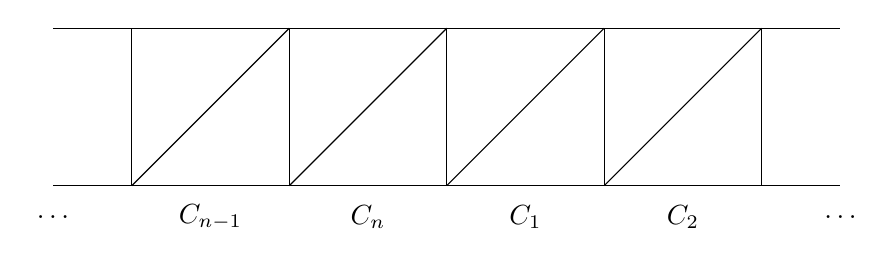
\begin{tikzpicture}
\draw (-5,1) -- (5,1);
\draw (-5,-1) -- (5,-1);

\foreach \x in {-4,-2,...,4}
\draw (\x,1) -- (\x,-1);

\foreach \x in {-4,-2,...,2}
\draw (\x,-1) -- (\x+2, 1);

\node at (-5,-1.4) {$\dots$};
\node at (-3,-1.4) {$C_{n-1}$};
\node at (-1,-1.4) {$C_{n}$};
\node at (1,-1.4) {$C_{1}$};
\node at (3,-1.4) {$C_{2}$};
\node at (5,-1.4) {$\dots$};
\end{tikzpicture}
\]
\[
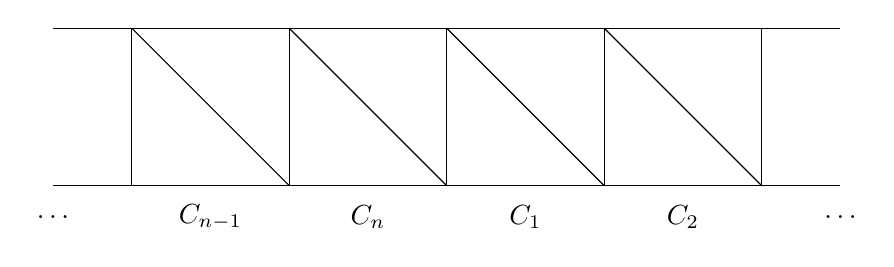
\begin{tikzpicture}
\draw (-5,1) -- (5,1);
\draw (-5,-1) -- (5,-1);

\foreach \x in {-4,-2,...,4}
\draw (\x,1) -- (\x,-1);

\foreach \x in {-4,-2,...,2}
\draw (\x,1) -- (\x+2, -1);

\node at (-5,-1.4) {$\dots$};
\node at (-3,-1.4) {$C_{n-1}$};
\node at (-1,-1.4) {$C_{n}$};
\node at (1,-1.4) {$C_{1}$};
\node at (3,-1.4) {$C_{2}$};
\node at (5,-1.4) {$\dots$};
\end{tikzpicture}
\]

Notice that in both cases the choice of diagonal is consistent throughout the band. We will say a band is \emph{positively oriented} if it is arranged as in the first figure and \emph{negatively oriented} otherwise. We require that the only adjacency relations between squares in a band are the ones expressed by the figures, so in particular bands have well-defined top and bottom sides. We remark that two differently oriented bands may intersect as the following figure shows: 

\begin{figure}[h]
\centering
\begin{tikzpicture}[scale=.65]
\foreach \x in {-4,-2,...,4}
{
\DSquare{\x}{0}
\DSquare{0}{\x}
}
\draw (-1, -6) to (-1, -5);
\draw (1, -6) to (1, -5);
\draw (-1, 6) to (-1, 5);
\draw (1, 6) to (1, 5);
\draw (-6,-1) to (-5,-1);
\draw (-6,1) to (-5,1);
\draw (6,-1) to (5,-1);
\draw (6,1) to (5,1);
\end{tikzpicture}
\caption{Two intersecting bands.}
\label{band-intersection}
\end{figure}

Given a surface $\Sigma$ of arbitrary genus, we consider families of loops $R=\{r_i\}$ and $B=\{b_j\}$ on $\Sigma$ satisfying the conditions stated in Proposition \ref{surface-loops}. We can now pick suitably small tubular neighborhoods of each loop and place a positively (resp. negatively) oriented band over each neighborhood corresponding to a loop in $R$ (resp. $B$). Conditions 1 and 2 of Proposition \ref{surface-loops} guarantee that all intersections between bands resemble that of figure \ref{band-intersection}. Condition 3 guarantees that each connected component of the complement of the bands is a polygon. We will refer to these polygons as \emph{regions}. Therefore, the collection of bands and regions actually define a polygonal subdivision of $\Sigma$. For technical reasons that will be clearer later, we will require each band to have at least 5 squares between any pair of intersections with other bands. This can be easily achieved by refining the division of the band if necessary. We will refer to this hypothesis as $(\diamond)$ throughout this section. From now on we fix a subdivision as described above for each genus $g$ and call its associated QP $(Q_g,P_g)$. The corresponding Jacobian algebra will be denoted $A_g$.

\marginpar{todas las figuras grandes de esta sección están escaladas para no romper el formato de los párrafos que siguen}
\begin{figure}[h]
\[
\begin{tikzpicture}[scale=0.5]
\foreach \x in {-6,-4,...,6}
{
\ArrowedSquare{\x}{6}
\ArrowedSquare{\x}{-6}
\ArrowedSquare{6}{\x}
\ArrowedSquare{-6}{\x}
}
\draw (-8,-7) to (-7,-7);
\draw (-8,-5) to (-7,-5);
\draw (8,-7) to (7,-7);
\draw (8,-5) to (7,-5);
\draw (-8,7) to (-7,7);
\draw (-8,5) to (-7,5);
\draw (8,7) to (7,7);
\draw (8,5) to (7,5);
\draw (-7,-8) to (-7,-7);
\draw (-5,-8) to (-5,-7);
\draw (-7,8) to (-7,7);
\draw (-5,8) to (-5,7);
\draw (7,-8) to (7,-7);
\draw (5,-8) to (5,-7);
\draw (7,8) to (7,7);
\draw (5,8) to (5,7);
\foreach \x in {-4,-2,...,2}
{
\draw[<-, red, very thick] (-6+1.1, \x + 0.1) to [bend right] (-6+1.1, \x + 1.9);
\draw[->, red, very thick] (6-1.1, \x + 0.1) to [bend left] (6-1.1, \x + 1.9);
\draw[->, red, very thick] (\x + 0.1,-6+1.1) to [bend left] (\x + 1.9,-6+1.1);
\draw[<-, red, very thick] (\x + 0.1, 6-1.1) to [bend right] (\x + 1.9, 6-1.1);
}
\draw[->, red, very thick] (-4-0.1, 6-1.1) to [bend left] (-6+1.1, 4+0.1);
\draw[<-, red, very thick] (4+0.1, 6-1.1) to [bend right] (6-1.1, 4+0.1);
\draw[<-, red, very thick] (6-1.1, -4-0.1) to [bend right] (4+0.1, -6+1.1);
\draw[->, red, very thick] (-6+1.1, -4-0.1) to [bend left] (-4-0.1,-6+1.1);
\end{tikzpicture}
\]
\caption{The configuration of the associated quiver $Q_g$ around a region satisfying $(\diamond)$.}
\end{figure}
We now turn to the study of some relations that hold in $A_g$, that will enable us to prove its finite-dimensionality.

\begin{lemma}\label{band-sides} Any path in $A_g$ passing through vertices of both sides of a band is zero.
\end{lemma}
\begin{proof} Throughout this and the following proofs, we will only consider our bands to be positively oriented, since the analogous statements for negatively oriented bands are proved in a similar fashion. We name the arrows in the quiver as in the following figure:
\[
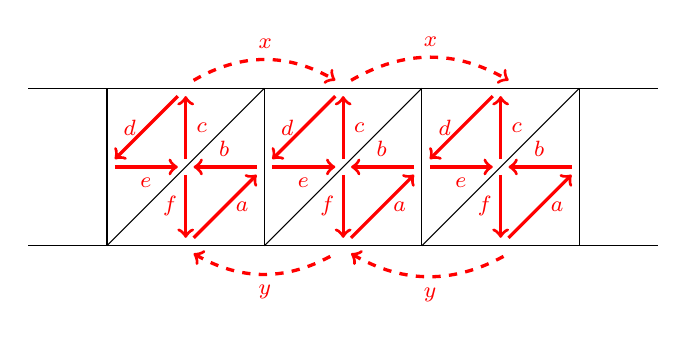
\begin{tikzpicture}[text width=1.5mm, font=\footnotesize]
\draw (-4, 0) -- (4, 0);
\draw (-4, 2) -- (4, 2);
\foreach \x in {-3,-1,...,3}
\draw (\x, 0) -- (\x, 2);
\foreach \x in {-3,-1,1}
{
\draw (\x,0) -- (\x+2, 2);
\draw [->, red, very thick] (\x+1.9, 1) to node[above] {$b$} (\x+1.1, 1);
\draw[->, red, very thick] (\x+1, 0.9) to node[left]{$f$} (\x+1, 0.1);
\draw[->, red, very thick] (\x+1.1, 0.1) to node[right]{$a$} (\x+1.9, 0.9);
\draw[->, red, very thick] (\x+1, 1.1) to node[right]{$c$} (\x+1, 1.9);
\draw[->, red, very thick] (\x+0.9, 1.9) to node[left]{$d$} (\x+0.1, 1.1);
\draw[->, red, very thick] (\x+0.1, 1) to node[below]{$e$} (\x+0.9, 1);
}

\draw[->, red, dashed, very thick] (-1.9, 2.1) to [bend left] node[above]{$x$} (-0.1, 2.1);
\draw[->, red, dashed, very thick] (0.1, 2.1) to [bend left] node[above]{$x$} (2.1, 2.1);
\draw[<-, red, dashed, very thick] (-1.9, -0.1) to [bend right] node[below]{$y$} (-0.1, -0.1);
\draw[<-, red, dashed, very thick] (0.1, -0.1) to [bend right] node[below]{$y$} (2.1, -0.1);
\end{tikzpicture}
\]

Since our quiver arises from a polygonal subdivision, we know that there is a cycle around each vertex,\marginpar{esto hay que probarlo en algún momento} and so each $x$ and each $y$ are paths of length at least 1. We mark those paths in the figure with a dashed arrow. We have given the same name to arrows occupying the same position in different squares, since this abuse of notation will be useful for calculation.

Inspecting the figure we see that any path passing through vertices of both sides of the band must contain a path of the form $cba$ or $fed$ as factors. It suffices to check that both of them are zero in $A_g$.

We have that $\partial_f(P_g) = ba + eay$, and so $ba  = -eay$ in $A_g$. Therefore, we have that $cba = -ceay$. Moreover, $\partial_d(P_g) = ce + xcb$, from which we deduce that $ce = -xcb$ in $A_g$. Putting all of this together, we get that $cba=-ceay=xcbay$ (one should note that the $cba$ factor in the right hand side of the equality consists of arrows placed on the square immediately left from the one where we started). Proceeding inductively we get $cba=x^ncbay^n$ for all positive $n$. Since $x$ and $y$ are paths of length at least $1$, this shows that $cba$ is equal to paths of arbitrarily high length. Therefore, we conclude that $cba=0$ in $A_g$. \marginpar{esto también hay que hacerlo...}

An analogous argument shows that $fed=0$ in $A_g$ as well, concluding the proof. 
\end{proof}

\begin{lemma}\label{long-band-paths} Any sufficiently long path contained entirely in bands is zero in $A_g$. More precisely, any non-zero path contained in a single band (resp. several bands) is of length at most 5 (resp. 9).
\end{lemma}
\begin{proof} We first prove that any sufficiently long path cotained entirely in a single band is zero. As we have already seen, any path passing through vertices of both sides of the band is zero, so we will suppose without loss of generality that our path is placed on the upper part of the band. Mantaining the notation used on the proof of the previous lemma, this is equivalent to saying our path only has arrows $b, c, d$ or $e$ as factors.

We start by studying paths containing a $3$-cycle as a prefix. The $3$-cycles $edc$ and $ced$ only prefix two paths of length 4, namely $cedc$ and $dced$. Since $\partial_e(P_g) = dc + ayf$, the relation $dc = -ayf$ holds, and so $cedc=-ceayf=0$ and $dced=-ayfed=0$ by Lemma \ref{band-sides}. Moreover, the $3$-cycle $dce$ only prefixes two paths of length 5, which are $cbdce$ and $cedce$. Clearly, $cedce=0$ since we have already shown that $cedc=0$, and using the relation $dc=-ayf$ we get $cbdce = - cbayfe=0$ once again by Lemma \ref{band-sides}.

Now we turn to paths containing a $3$-cycle as a suffix. Once again, the $3$-cycles $ced$ and $dce$ only suffix two paths of length 4, which are $cedc$ and $dced$, already shown to be zero previously. The $3$-cycle $edc$ is a suffix to only two paths of length 5, which are $edcbd$ and $edced$. We see that $edced=0$ since $dced=0$ and $edcbd=-eayfbd=0$ as we wanted.

Therefore, any path in a band of length $>5$ containing a 3-cycle is zero, since we have shown these cycles only admit prefixes and suffixes of length at most 1.

Now, a path of length $>5$ not containing a 3-cycle is either of the form $dcbdcb$, $bdcbdc$ or $cdbcbd$. All possibilites have $cbdc$ as a factor, which is clearly zero since $cbdc = -cbayf = 0$ by Lemma \ref{band-sides}. Therefore, we conclude that any path of length $>5$ contained in a single band is zero.

Finally, consider a path of length $>9$ contained in possibly different bands. If its first six arrows lie on the same band, the path is zero as seen previously. Otherwise, at most five of its first arrows lie on the same band and the sixth is then placed on a different band intersecting the original one, as seen in the following figure:
\[
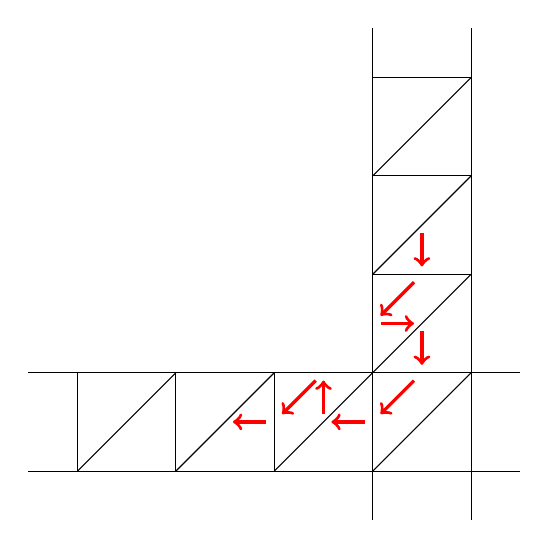
\begin{tikzpicture}
\draw (-3.5*1.25, 0) -- (1.5*1.25, 0);
\draw (-3.5*1.25, -1.25) -- (1.5*1.25, -1.25);
\draw (0,3.5*1.25) -- (0,-1.5*1.25);
\draw (1.25,3.5*1.25) -- (1.25,-1.5*1.25);

\foreach \x in {-3.75,-2.5,...,0}
{
\draw (\x,-1.25) -- (\x+1.25, 0);
\draw (0, -\x) -- (1.25, -\x);
\draw (\x,0) -- (\x, -1.25);
}

\foreach \x in {0,1.25,...,2.5}
\draw (0, \x) -- (1.25, \x+1.25);

\draw[->, red, very thick] (0.5*1.25, 1.5*1.25 - 0.1) -- (0.5*1.25, 1.25 + 0.1);
\draw[->, red, very thick] (0.5*1.25 - 0.1, 1.25-0.1) -- (0.1, 0.5*1.25+0.1);
\draw[->, red, very thick] (0.1, 0.5*1.25) -- (0.5*1.25 - 0.1, 0.5*1.25);
\draw[->, red, very thick] (0.5*1.25, 0.5*1.25-0.1) -- (0.5*1.25, 0.1);
\draw[->, red, very thick] (0.5*1.25 - 0.1, -0.1) -- (0.1, -0.5*1.25+0.1);
\draw[->, red, very thick] (-0.1, -0.5*1.25) -- (-0.5*1.25+0.1, -0.5*1.25);
\draw[->, red, very thick] (-0.5*1.25, -0.5*1.25+0.1) -- (-0.5*1.25, -0.1);
\draw[->, red, very thick] (-0.5*1.25 - 0.1, -0.1) -- (-1.25 + 0.1, -0.5*1.25+0.1);
\draw[->, red, very thick] (-1.25 -0.1, -0.5*1.25) -- (-1.5*1.25+0.1, -0.5*1.25);
\end{tikzpicture}
\]

Since by hypothesis $(\diamond)$ \marginpar{quizás podria haber un link a la def de $\diamond$}two intersections in the same band are distanced by at least five squares, we conclude that at least the next six arrows belong to the same band. Therefore, any path of length $>9$ contained entirely in bands is zero in $A_g$, as we wanted.
\end{proof}

\begin{lemma}\label{long-region-paths} Any non-zero path entirely contained in an $n$-sided region is of length at most $3n-4$.
\end{lemma}
\begin{proof} We fix an $n$-sided region. Consider any band neighboring our region and pick any of its squares that is at least two squares away from an intersection with another band, which is always possible by hypothesis $(\diamond)$. Recalling the fact that our region induces an $n$-cycle in the quiver, we name the arrow starting at the square we picked as $x_0$. In general, given $j\in \ZZ/n\ZZ$ we call $x_j$ the arrow starting at the target of $x_{j-1}$. Keeping the previous notation for arrows contained in bands, our current situation is illustrated by this figure:
\[
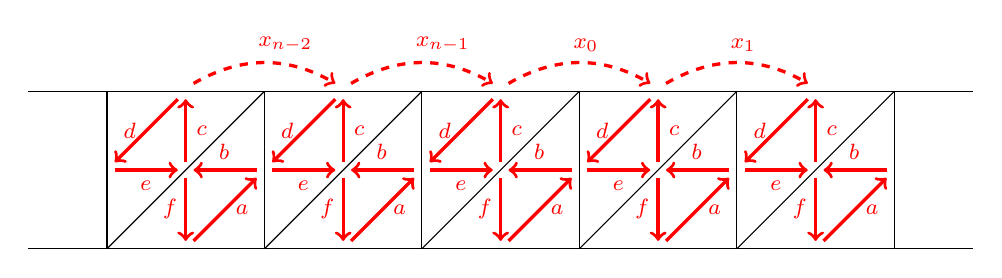
\begin{tikzpicture}[text width=1.5mm, font=\footnotesize]
\draw (-6, 0) -- (6, 0);
\draw (-6, 2) -- (6, 2);
\foreach \x in {-5,-3,...,5}
\draw (\x, 0) -- (\x, 2);
\foreach \x in {-5,-3,...,3}
{
\draw (\x,0) -- (\x+2, 2);
\draw [->, red, very thick] (\x+1.9, 1) to node[above] {$b$} (\x+1.1, 1);
\draw[->, red, very thick] (\x+1, 0.9) to node[left]{$f$} (\x+1, 0.1);
\draw[->, red, very thick] (\x+1.1, 0.1) to node[right]{$a$} (\x+1.9, 0.9);
\draw[->, red, very thick] (\x+1, 1.1) to node[right]{$c$} (\x+1, 1.9);
\draw[->, red, very thick] (\x+0.9, 1.9) to node[left]{$d$} (\x+0.1, 1.1);
\draw[->, red, very thick] (\x+0.1, 1) to node[below]{$e$} (\x+0.9, 1);
}

\draw[->, red, dashed, very thick] (-5+1.1, 2.1) to [bend left] node[above]{$\mathclap{x_{n-2}}$} (-5+2.9, 2.1);
\draw[->, red, dashed, very thick] (-3+1.1, 2.1) to [bend left] node[above]{$\mathclap{x_{n-1}}$} (-3+2.9, 2.1);
\draw[->, red, dashed, very thick] (-1+1.1, 2.1) to [bend left] node[above]{$\mathclap{x_{0}}$} (-1+2.9, 2.1);
\draw[->, red, dashed, very thick] (1+1.1, 2.1) to [bend left] node[above]{$\mathclap{x_{1}}$} (1+2.9, 2.1);
\end{tikzpicture}
\]

We now prove that the path $L=x_{n-1}x_{n-2}\dots x_2x_1x_{0}x_{n-1}\dots x_3x_2$ is zero. We have that $\partial_{x_0}(P_g)=x_{n-1}x_{n-2}\dots x_2x_1+cbd$ and $\partial_{x_1}(P_g)=x_{0}x_{n-1}\dots x_3x_2+cbd$. Therefore, the relations
\begin{align*}
x_{n-1}x_{n-2}\dots x_2x_1=-cbd\\
x_{0}x_{n-1}\dots x_3x_2=-cbd
\end{align*}
hold in $A_g$. We stress that $cbd$ denotes a different path in each one of the two equations: they are similar paths contained in different squares. Using these relations, we see that $$x_{n-1}x_{n-2}\dots x_2x_1x_{0}x_{n-1}\dots x_3x_2=-cbdx_{0}x_{n-1}\dots x_3x_2=cbdcbd,$$ and the latter is zero by Lemma \ref{long-band-paths} since $cbdcbd$ is a path of length 6 lying on a single band. 

Finally, since the longest path entirely contained in our region not having $L$ as a factor is
\[\underbrace{x_{n-2}x_{n-1}\dots x_0}_{\text{$n-1$ arrows}}\underbrace{x_{n-1}x_{n-2}\dots x_0}_{\text{$n$ arrows}}\underbrace{x_{n-1}x_{n-2}\dots x_3}_{\text{$n-3$ arrows}},\]
which is of length $3n-4$, the result follows.
\end{proof}

\begin{lemma} \label{long-br-paths} Any sufficiently long path not having factors from two different regions is zero in $A_g$.
\end{lemma}
\begin{proof} We write our path as $B_{k+1}R_k\dots R_2 B_2 R_1 B_1$, where the paths $R_i$ are contained in a same region and the paths $B_j$ are non-trivial (except possibly for $B_1$ and $B_{k+1}$) and contained in bands.

Let $1<j<k+1$. The path $B_j$ starts and ends at the boundary of our region of interest. Therefore, it must pass through both of the endpoints of a same arrow belonging to the cycle associated to the region, which we will call $x_0$ following the notation employed in the proof of Lemma \ref{long-band-paths}.\marginpar{esto no está particularmente claro...} Therefore, using the relation induced by $\partial_{x_0}(P_g)$, we can replace some of the arrows in $B_j$ with a path entirely contained in the region.
After applying this argument repeatedly, we can then suppose our path is of the form $B_2 R_1 B_1$. The proof now follows from Lemmas \ref{long-band-paths} and \ref{long-region-paths}, since if our path is non-zero, then $|B_1|<10$, $|B_2|<10$ and $|R_1|<3n-3$, where $n$ is the number of sides of the region.
\end{proof}

After proving all these lemmas, the main result of this section now easily follows:

\begin{thm} The algebra $A_g$ is finite-dimensional.
\end{thm}
\begin{proof} By Lemma \ref{long-br-paths}, any sufficiently long path is zero if it does not have factors from two different regions, but any path that does must be zero (regardless of length) by Lemma \ref{band-sides}, since it must cross a band. Therefore, any sufficiently long path is zero, and so $A_g$ is finite-dimensional.
\end{proof}
\end{section}

\begin{section}{A family of infinite-dimensional examples}
We now turn to the study of another family of polygonal subdivisions, this time inducing infinite-dimensional algebras. 

Let $n>2$. We say that a polygonal subdivision of a surface $\Sigma$ is \emph{$n$-regular} if all of its faces have exactly $n$ sides and exactly $n$ faces meet at every vertex. For example, a tetrahedron is a $3$-regular subdivision of the sphere, and the following figures induce $4$-regular subdivisions of the torus after identifying the opposing sides of each square:
\[
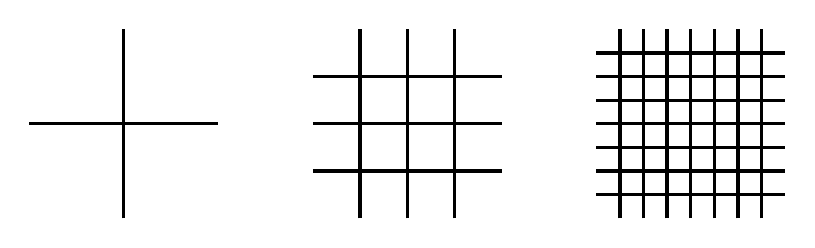
\begin{tikzpicture}[scale=1.2, very thick]
\Square{-3}{0}
\Square{0}{0}
\Square{3}{0}
\draw (-3,-1) to (-3,1);
\draw (-4,0) to (-2,0);

\foreach \x in {-0.5,0,0.5}
{
\draw (\x, -1) to (\x, 1);
\draw (-1, \x) to (1, \x);
}

\foreach \x in {-0.75,-0.5, ..., 0.75}
{
\draw (3+\x, -1) to (3+\x, 1);
\draw (2, \x) to (4, \x);
}
\end{tikzpicture}
\]
Obviously, in this way one can produce an infinite number of these examples on the torus.

The existence of an $n$-regular subdivision imposes strong conditions on the surface. In fact, suppose we have an $n$-regular subdivision of a surface and let $v, e$ and $f$ denote its number of vertices, edges and faces respectively. Since every face contains exactly $n$ vertices and every vertex belongs to exactly $n$ faces, we have that $v=f$. Moreover, every face contains $n$ edges and any edge belongs to exactly 2 faces, so $e=nf/2$.
Recalling the fact that the Euler characteristic of a surface of genus $g$ is $2-2g$, we have that $2-2g=v-e+f=(2-n/2)f$, or equivalently $4g-4 = (n-4)f$. If $n=4$, the right hand vanishes, and so $g=1$. Therefore, the only surface that can admit a $4$-regular subdivision is the torus (and in fact we have already shown there are an infinite number of them).

Suppose now that $n\neq 4$. Then \[f=\frac{4g-4}{n-4},\] and so $g$ must be such that this quotient is integral. Moreover, since $n$ faces meet at every vertex, there must be at the very least $n$ faces, and so $n(n-4)\leq 4(g-1)$. Therefore, we have that $g\in \Omega(n^2)$.\marginpar{no se si vale la pena observar esto}

All of these are \emph{necessary} conditions for an $n$-regular subdivision to exist. Although at first they may appear to be too restrictive, in fact there exist surfaces $\Sigma_n$ admitting $n$-regular subdivisions for all $n>2$. \marginpar{\textcolor{red}{completar esto cuando lo tengamos, si es que es cierto :)}}

Our main interest in the concept of $n$-regularity lies in the following fact:

\begin{thm} The Jacobian algebra associated to an $n$-regular subdivision of a surface is infinite-dimensional.
\end{thm}
\begin{proof} Let $(Q,P)$ be the quiver with potential associated to the subdivision, $I$ the ideal in $\kQ$ spanned by the cyclic derivatives of the potential $P$ and $J$ the closure of $I$ in $\KQ$. The inclusion $i:\kQ\to \KQ$ induces a monomorphism $i:\kQ/I \to \KQ/J$, so it suffices to see that $\kQ/I$ is infinite-dimensional. \marginpar{no recuerdo por qué valía esto}

Any arrow $x$ in the quiver is a factor of exactly two cycles in $P$: one of them is contained in the same face of the subdivision as $x$ and the other surrounds a vertex and is composed of arrows lying in different faces.\marginpar{esto hay que probarlo con más detalle en los preliminares} The condition of $n$-regularity forces these two cycles to be of length $n$, and so $\partial_x(P)= a+b$, with $a$ and $b$ paths of length $n-1$. Therefore, $I$ is an homogeneous ideal, since it is spanned by homogeneous elements, and so $\kQ/I$ inherits a grading from $\kQ$. \marginpar{quedó medio chueca la figura siguiente:}
\begin{figure}[h]
\[
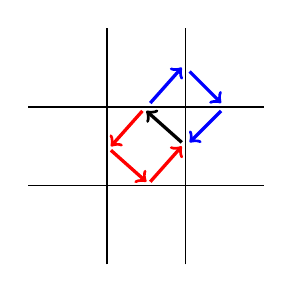
\begin{tikzpicture}[scale=0.5]
\draw (-3,1) to (3,1);
\draw (-3, -1) to (3, -1);
\draw (-1, -3) to (-1, 3);
\draw (1, -3) to (1, 3);
\draw[very thick, ->] (0.9, 0.1) to (0, 0.9);
\draw[red, very thick, ->] (-0.1, 0.9) to (-0.9, 0);
\draw[red, very thick, ->] (-0.9, -0.1) to (0, -0.9);
\draw[red, very thick, ->] (0.1, -0.9) to (0.9, 0);
\draw[blue, very thick, ->] (0.1, 1.1) to (0.9, 2);
\draw[blue, very thick, ->] (1.1, 1.9) to (1.9, 1.1);
\draw[blue, very thick, ->] (1.9, 0.9) to (1.1, 0.1);
\end{tikzpicture}
\]
\begin{caption}{Any cyclic derivative of the potential $P$ associated to a 4-regular subdivision turns out to be of the form $\textcolor{red}{a} + \textcolor{blue}{b}$, with both $\textcolor{red}{a}$ and $\textcolor{blue}{b}$ of length 3.}
\end{caption}
\end{figure}

The path algebra $\kQ$, regarded as a $k$-vector space, admits a direct sum decomposition $A\oplus B$, where $A$ is the subspace spanned by paths 

$(\clubsuit)$ containing either $n-1$ consecutive arrows belonging to the same face or $n-1$ consecutive arrows surrounding the same vertex of the subdivision as factors \marginpar{arreglar el formato, debería ir en un párrafo aparte con un entorno especial, al igual que $(\diamond)$}

and $B$ is the subspace spanned by paths not satisfying $(\clubsuit)$. One immediately checks that $A$ is actually an ideal in $\kQ$. Even more, since every cyclic derivative is the sum of two paths satisfying $(\clubsuit)$, we have that $I\subseteq A$. Therefore, any non-zero path $c\in B$ is not contained in $I$, and in turn is not zero in $\kQ/I$.

Suppose now that $X$ is an infinite subset of $B$ composed of non-zero paths, all of different lengths. Since paths are homogeneous elements of $\kQ$ and $I$ is an homogeneous ideal, the projection of a path into $\kQ/I$ is an homogeneous element too. Therefore, the projection of $X$ to $\kQ/I$ is an infinite linearly independent set, since it is composed of non-zero homogeneous elements, each belonging to a different \textcolor{red}{why?} homogeneous component. So finally, all that remains to show is that one can actually produce such a set $X$.

\textcolor{red}{Para fabricar $X$ primero construimos un ciclo en $B$ y después simplemente tomamos sus potencias. Para armar un ciclo, tomo un camino construido de la siguiente manera: parto de una cara y me muevo dos flechas dentro de la cara, después salgo y recorro dos flechas dentro de una cara adyacente, nuevamente salgo y recorro otras dos y así siguiendo. Como el quiver es finito, eventualmente voy a obtener un ciclo con este procedimiento, y por construcción verifica que está en $B$. El problema es que el punto donde se pegan el principio y el final del ciclo pueden pertenecer a la misma cara (o rodear el mismo vértice) y así tener hasta 4 caminos consecutivos en la misma cara. Por lo tanto al tomar potencias me salgo de $B$ si $n<6$. Esto se puede arreglar a mano en el caso del toro por ejemplo, porque uno puede exhibir un $X$ específico (las potencias del zigzag), pero estaría bueno dar una construcción general. Además, ningún $X$ puede producirse para el tetraedro, porque no hay caminos de longitud $>2$ ahí que no verifiquen $(\clubsuit)$.}
\end{proof}
\end{section}
\end{chapter}